\documentclass[%
%  reprint,
superscriptaddress,
% groupedaddress,
%unsortedaddress,
% runinaddress,
% frontmatterverbose, 
% preprint,
%preprintnumbers,
%nofootinbib,
%nobibnotes,
%bibnotes,
 amsmath,amssymb,
%aps,
prl,
%pra,
prb,
% rmp,
%prstab,
% prstper,
%floatfix,
]{revtex4-2}


\usepackage{graphicx}% Include figure files
\usepackage{dcolumn}% Align table columns on decimal point
\usepackage{bm}% bold math
\usepackage{blindtext}
\usepackage{float}
\usepackage{caption}
\usepackage{cleveref}
\usepackage{subcaption}
\usepackage{xcolor}

\newcommand{\etal}{{\it et al.}~}
\newcommand{\bom}{\boldsymbol{\omega}}
\newcommand{\hel}{\textsuperscript{4}He }

\def\red#1{\textcolor{red}{#1}}
\def\blue#1{\textcolor{blue}{#1}}
\def\magenta#1{\textcolor{magenta}{#1}}
\newcommand*{\NOTE}[1]{\textbf{\color{red}[#1]}}

\def \s{\mathbf{s}}
\def \v{\mathbf{v}}
\def \x{\mathbf{x}}
\def \r{\mathbf{r}}
\def \k{\mathbf{k}}

\def \cm{\mathrm{cm}}
\def \cms{\mathrm{cm/s}}
\def \sec{\mathrm{s}}
\def \K{\mathrm{K}}

\def\red{\textcolor{red}}


\begin{document}
\preprint{APS/123-QED}

\title{Supplementary Materials: Inverse energy transfer in finite-temperature superfluid vortex reconnections}

\author{P. Z. Stasiak}
\affiliation{School of Mathematics, Statistics and Physics, Newcastle University, Newcastle upon Tyne, NE1 7RU, United Kingdom}

\author{C.F. Barenghi}
\author{A. Baggaley}
\affiliation{School of Mathematics, Statistics and Physics, Newcastle University, Newcastle upon Tyne, NE1 7RU, United Kingdom}



\author{L. Galantucci}
\affiliation{Istituto per le Applicazioni del Calcolo ``M. Picone" IAC CNR, Via dei Taurini 19, 00185 Roma, Italy}

\author{G. Krstulovic}
\affiliation{Universit\'e C\^ote d'Azur, Observatoire de la C\^ote d'Azur, CNRS,Laboratoire Lagrangre, Boulevard de l'Observatoire CS 34229 - F 06304 NICE Cedex 4, France}


\maketitle

\section{Numerical Method}

\begin{figure}
	\centering
	\begin{subfigure}[b]{0.49\textwidth}
		\centering
		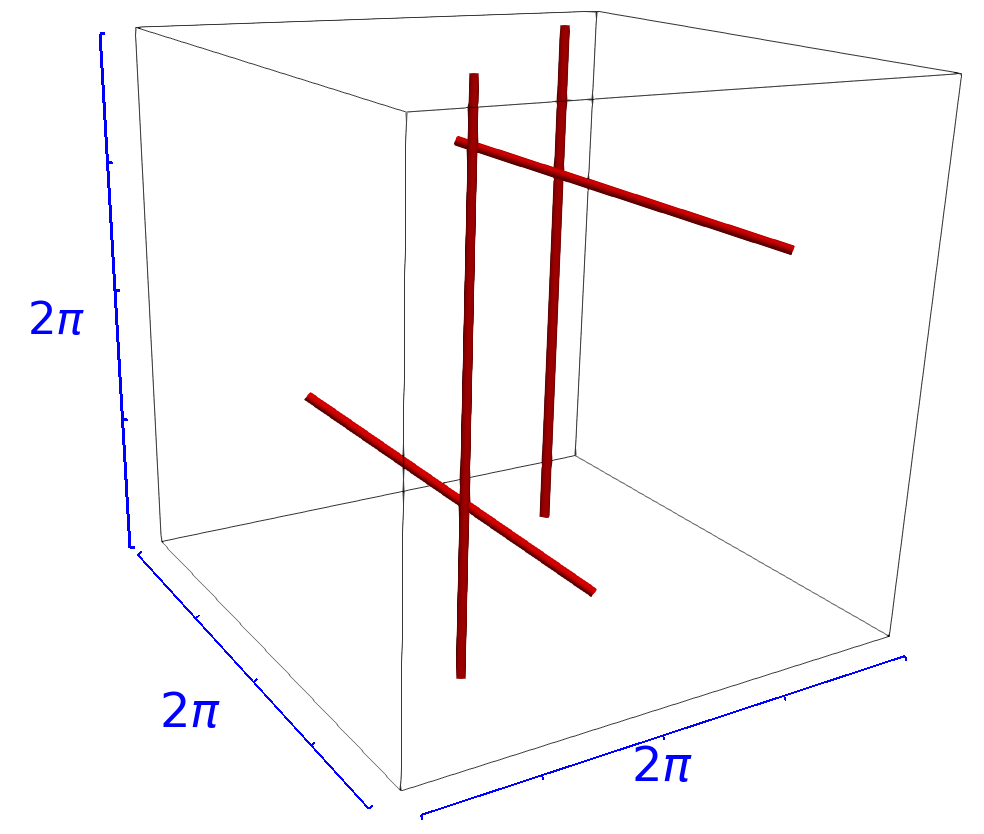
\includegraphics[width=0.8\textwidth]{schematic.png}
	\end{subfigure}
	\begin{subfigure}[b]{0.49\textwidth}
		\centering
		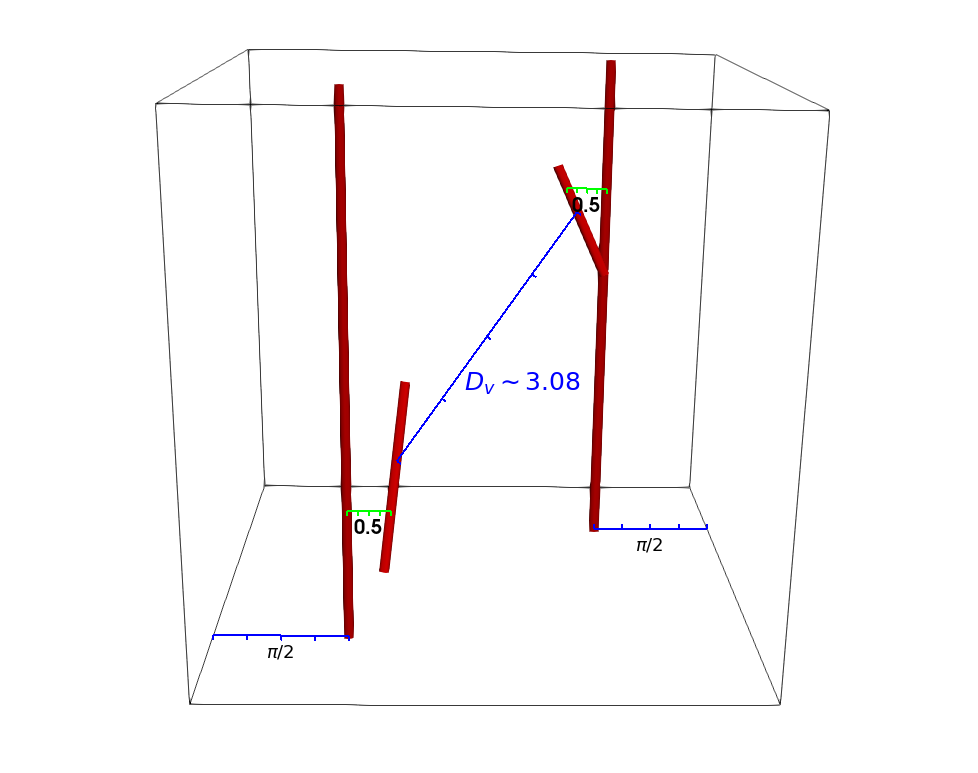
\includegraphics[width=0.9\textwidth]{schematic-2.png}
	\end{subfigure}
	\caption{Schematic diagram of the initial vortex configuration.}
	\label{fig:schematic}
\end{figure}

Using Schwarz mesoscopic model \cite{schwarzThreedimensionalVortexDynamics1988a}, vortex lines can be described as space curves $\s(\xi,t)$ of infinitesimal thickness, with a single quantum of circulation $\kappa=h/m_4=9.97\times10^{-8}\text{m}^2/\text{s}$, where $h$ is Planck's constant, $m_4=6.65\times10^{-27}\text{kg}$ is the mass of one helium atom, $\xi$ is the natural parameterisation, arclength, and $t$ is time. These conditions are a good approximation, since the vortex core radius of superfluid \textsuperscript{4}He($a_0=10^{-10}\text{m}$) is much smaller than any of the length scales of interest in turbulent flows. The equation of motion is
\begin{equation}
	\dot{\s}(\xi,t) = \v_s + \frac{\beta}{1+\beta}\left[\v_{ns}\cdot \s'\right]\s' + \beta\s'\times\v_{ns}+\beta'\s'\times\left[\s'\times \v_{ns}\right],
\end{equation}
where $\dot{\s}=\partial\s/\partial t$, $\s'=\partial\s/\partial \xi$ is the unit tangent vector, $\v_{ns}=\v_n - \v_s$, $\v_n$ and $\v_s$ are the normal fluid and superfluid velocities at $\s$ and $\beta$,$\beta'$ are temperature and Reynolds number dependent mutual fricition coefficients \cite{galantucciNewSelfconsistentApproach2020b}. The superfluid velocity $\v_s$ at a point $\x$ is determined by the Biot-Savart law
\begin{equation}
	\v_s(\x,t) = \frac{\kappa}{4\pi}\oint_{\mathcal{T}}\frac{\s'(\xi,t)\times\left[\x-\s(\xi,t)\right]}{|\x-\s(\xi,t)|}d\xi,
\end{equation}
where $\mathcal{T}$ represents the entire vortex configuration.
There is currently a lack of a well-defined theory of vortex reconnections in superfluid helium, like for the Gross-Pitaevskii equation \cite{villoisIrreversibleDynamicsVortex2020,villoisUniversalNonuniversalAspects2017a,promentMatchingTheoryCharacterize2020a}. An \emph{ad hoc} vortex reconnection algorithm is employed to resolve the collisions of vortex lines \cite{baggaleySensitivityVortexFilament2012a}.

A \emph{two-way model} is crucial to understand the accurately interept the back-reaction effect of the normal fluid on the vortex line and vice-versa \cite{stasiakCrossComponentEnergyTransfer2024}. We self-consistently evolve the normal fluid $\v_n$ with a modified Navier-Stokes equation
\begin{equation}
	\frac{\partial \v_n}{\partial t} + (\v_n\cdot\nabla)\v_n = -\nabla\frac{p}{\rho} + \nu_n\nabla^2\v_n + \frac{\mathbf{F}_{ns}}{\rho_n},
\end{equation}
\begin{equation}
	\mathbf{F}_{ns} = \oint_{\mathcal{T}}\mathbf{f}_{ns}\delta(\x-\x)d\xi, \quad \nabla\cdot\v_n=0,
\end{equation}
where $\rho=\rho_n + \rho_s$ is the total density, $\rho_n$ and $\rho_s$ are the normal fluid and superfluid densities, $p$ is the pressure, $\nu_n$ is the kinematic viscosity of the normal fluid and $\mathbf{f}_{ns}$ is the local friction per unit length \cite{galantucciCoupledNormalFluid2015a}
\begin{equation}
	\mathbf{f}_{ns} = -\mathcal{D}\s'\times\left[\s'\times(\dot{\s}-\v_n)\right]-\rho_n\kappa\s'\times(\v_n-\dot{\s}), 
	\label{eq:mutual-friction}
\end{equation}
where $\mathcal{D}$ is a coefficient dependent on the vortex Reynolds number and intrinsic properties of the normal fluid. The regularisation of the mutual fricition force onto the normal fluid grid is physically motivated by the strongly localised injection of vorticity during the momentum exchange of point-like particles and viscous flow in classical fluid dynamics \cite{gualtieri2015exact,gualtieri2017turbulence}. In short, the localised vorticity induced by the relative motion between the vortex lines and the normal fluid is diffused to discretisation of the grid spacing $\Delta x$ in a time interval $\epsilon_R$. In this way, the delta-forced fricition as defined in Eq.~\ref{eq:mutual-friction} is regularised by a Gaussian function, the fundamental solution of the diffusion equation. Further details of the method for classical fluids are contained in \cite{gualtieri2015exact,gualtieri2017turbulence} and for FOUCAULT in \cite{galantucciNewSelfconsistentApproach2020b}.  

In this Letter, we report all results using dimensionless units, where the characteristic length scale is $\tilde{\lambda} = D/D_0$, where $D^3=(1\times10^{-3}\mathrm{m})^3$ is the dimensional cube size, $D_0^3=(2\pi)^3$ is the non-dimensional cubic computational domain. The time scale is given by $\tilde{\tau}=\tilde{\lambda}^2\nu_n^0\nu_n$, where the non-dimensional viscosity $\nu_n^0$ resolves the small scales of the normal fluid. In these simulations, these quanties are $\tilde{\lambda}=1.59\times10^{-4}$m, $\nu_n^0=0.32$ and $\tilde{\tau}=0.366$s at $T=1.9K$ and $\tilde{\tau}=0.485$s at $T=2.1K$. We consider an initial configuration of two pairs of orthongal vortices, initialised as shown in the schematic of Fig.~\ref{fig:schematic}. The seperation between vortices in each pair $d$ is set to be $d_v=0.5$ in dimensionless units, and the shortest distance between pairs is $D_v=\sqrt{(\pi-d_v/2)^2+\pi^2}\sim 3.08$, so that $d_v\ll D_v$. 

\bibliography{references}% Produces the bibliography via BibTeX.
\end{document}
